\documentclass[UTF8, twocolumn]{ctexart}

\newcommand{\mytitle}{循环神经网络\\Recurrent Neural Network}
\usepackage{graphicx}
\usepackage{booktabs}
\usepackage{colortbl}
\usepackage{enumerate}
\usepackage{enumitem} % Make Itemize Indent Zero
\usepackage{lineno}
\usepackage{amssymb}
\usepackage{amsmath}
\usepackage{framed}
\usepackage{subcaption}
\usepackage[colorlinks,linkcolor=red,anchorcolor=red,citecolor=red]{hyperref}
\usepackage{float}
\graphicspath{{figures/}}

\usepackage{geometry}
\geometry{a4paper,left=2cm,right=2cm,bottom=2.5cm}

\usepackage{fancyhdr}
% \setlength{\headheight}{1.1cm}

\pagestyle{fancy}
\fancyhf{}
\fancyhead[C]{循环神经网络}
\fancyhead[L]{\leftmark}
\fancyhead[R]{\thepage}
\renewcommand{\headrulewidth}{1pt}

\begin{document}
\title{\mytitle}
\author{A Note by DaweiX}
\date{}
\maketitle

\section{RNN}

\subsection{基本架构}
循环神经网络(Recurrent Neural Network, RNN)是一种用于处理序列数据的神经网络. 
一个RNN的基本单元可以表示为一个函数$f:h^{\prime}, y = f(h, x)$, 
如图\ref{rnn1}所示. 其中\footnote{本文中各式中均未加入偏置. 事实上, 为了方便
计算, 可以理解偏置已经包含在$W$中}

\begin{align}
h^{\prime} &= \sigma(W^h h + W^i x)\\
y &= \sigma(W^o h^{\prime})
\end{align}


\begin{figure}[!hbt]
    \center
    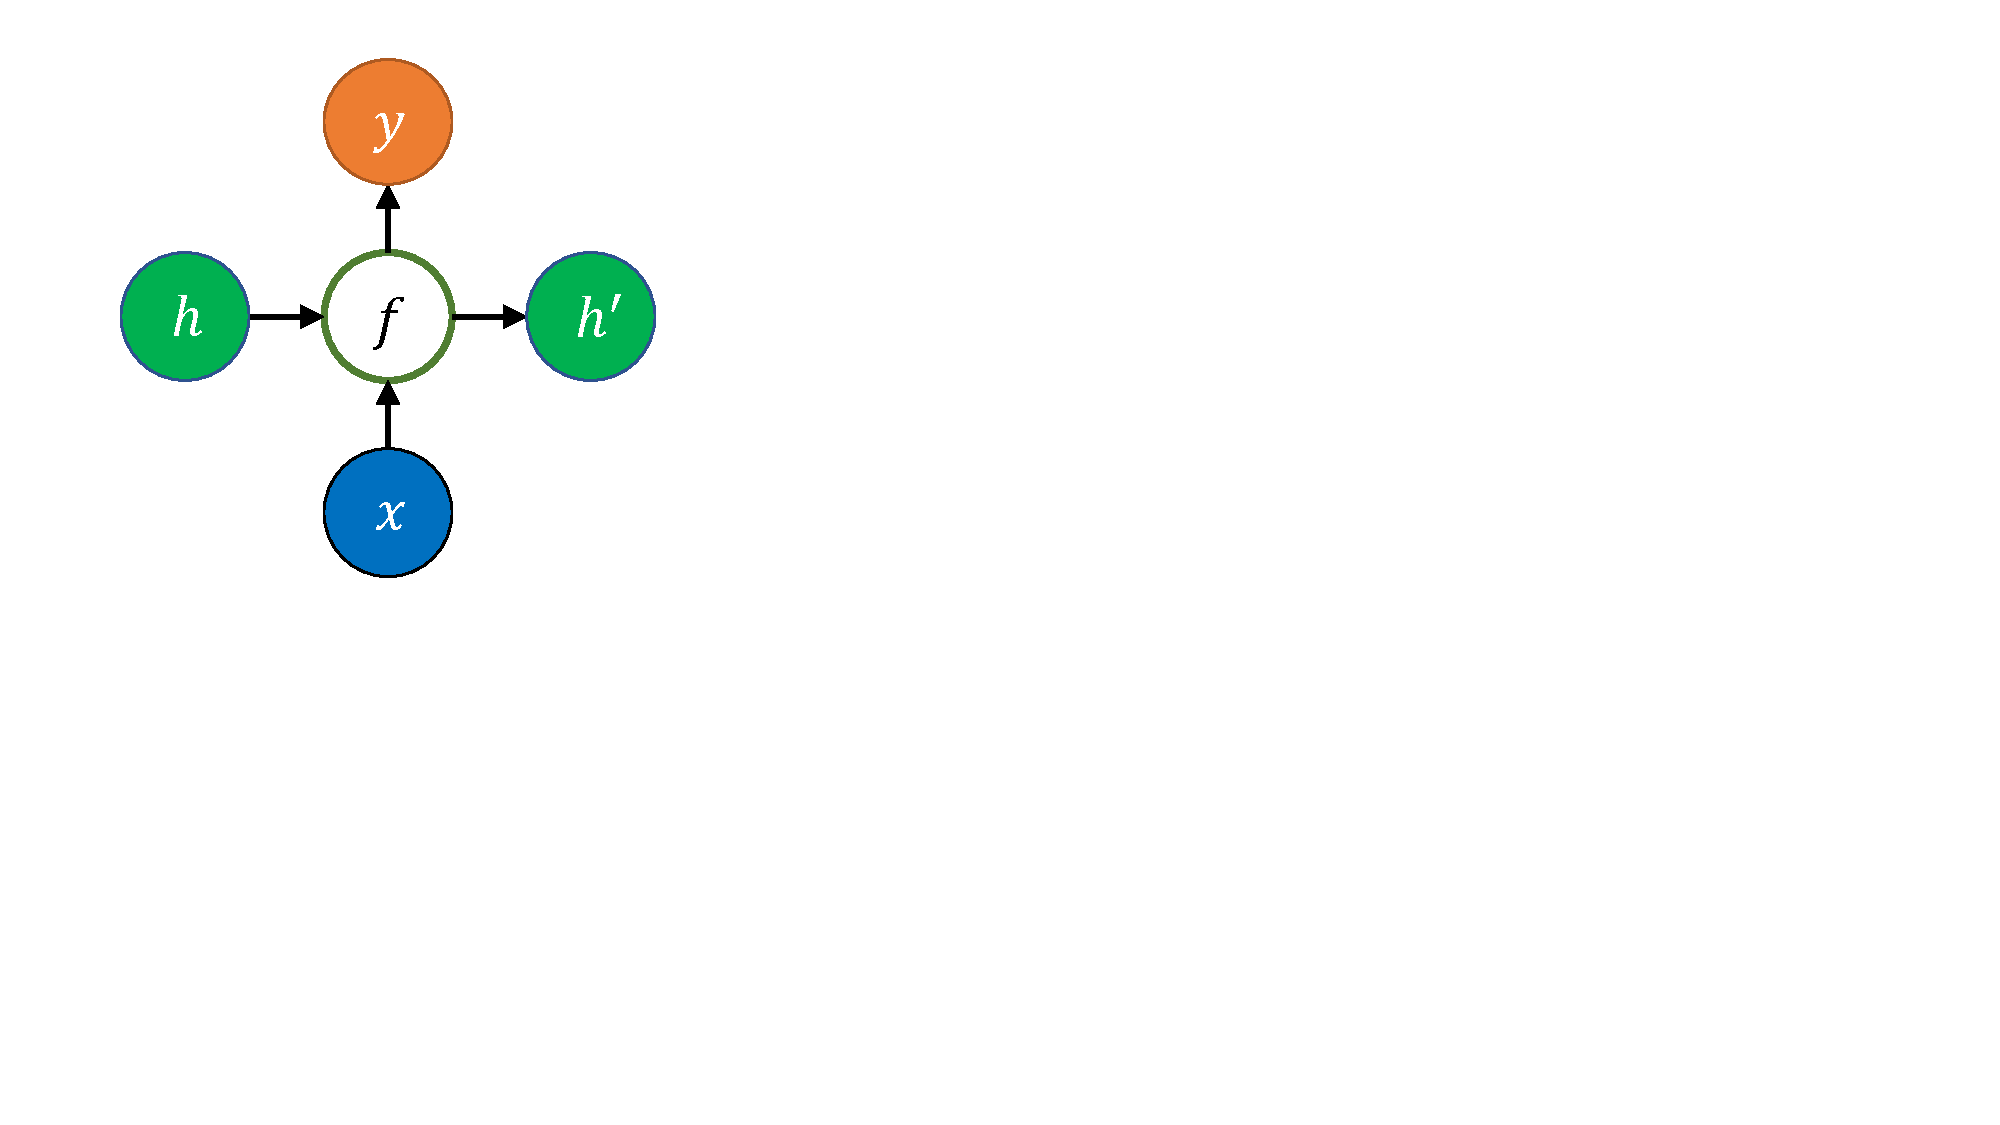
\includegraphics[width=.3\linewidth]{rnn1.pdf}
    \caption{RNN的一个基本单元}
    \label{rnn1}
\end{figure}

这里, $x$为当前状态下数据的输入, $h$表示接收到的上一个节点的输入. 
$y$为当前节点状态下的输出, 而$h^{\prime}$为传递到下一个节点的输出. 
通过上图的公式可以看到, 输出$h^{\prime}$与$x$和$h$的值都相关. 
而$y$则常常使用$h^{\prime}$投入到一个线性层(主要是进行维度映射), 
然后使用softmax进行分类得到需要的数据. 对这里的$y$, 
如何通过$h^{\prime}$计算得到往往看具体模型的使用方式. 通过序列形式的输入, 
我们能够得到如下形式的RNN. 图\ref{rnn2}右侧为左侧的简化版本. 其中, 从下到上的
三个节点分别相当于神经网络的输入层、隐含层以及输出层. 可以看到, 相比多层感知机, 
RNN隐含层中的各个神经元之间也带有权值. 


\begin{figure}[!hbt]
    \center
    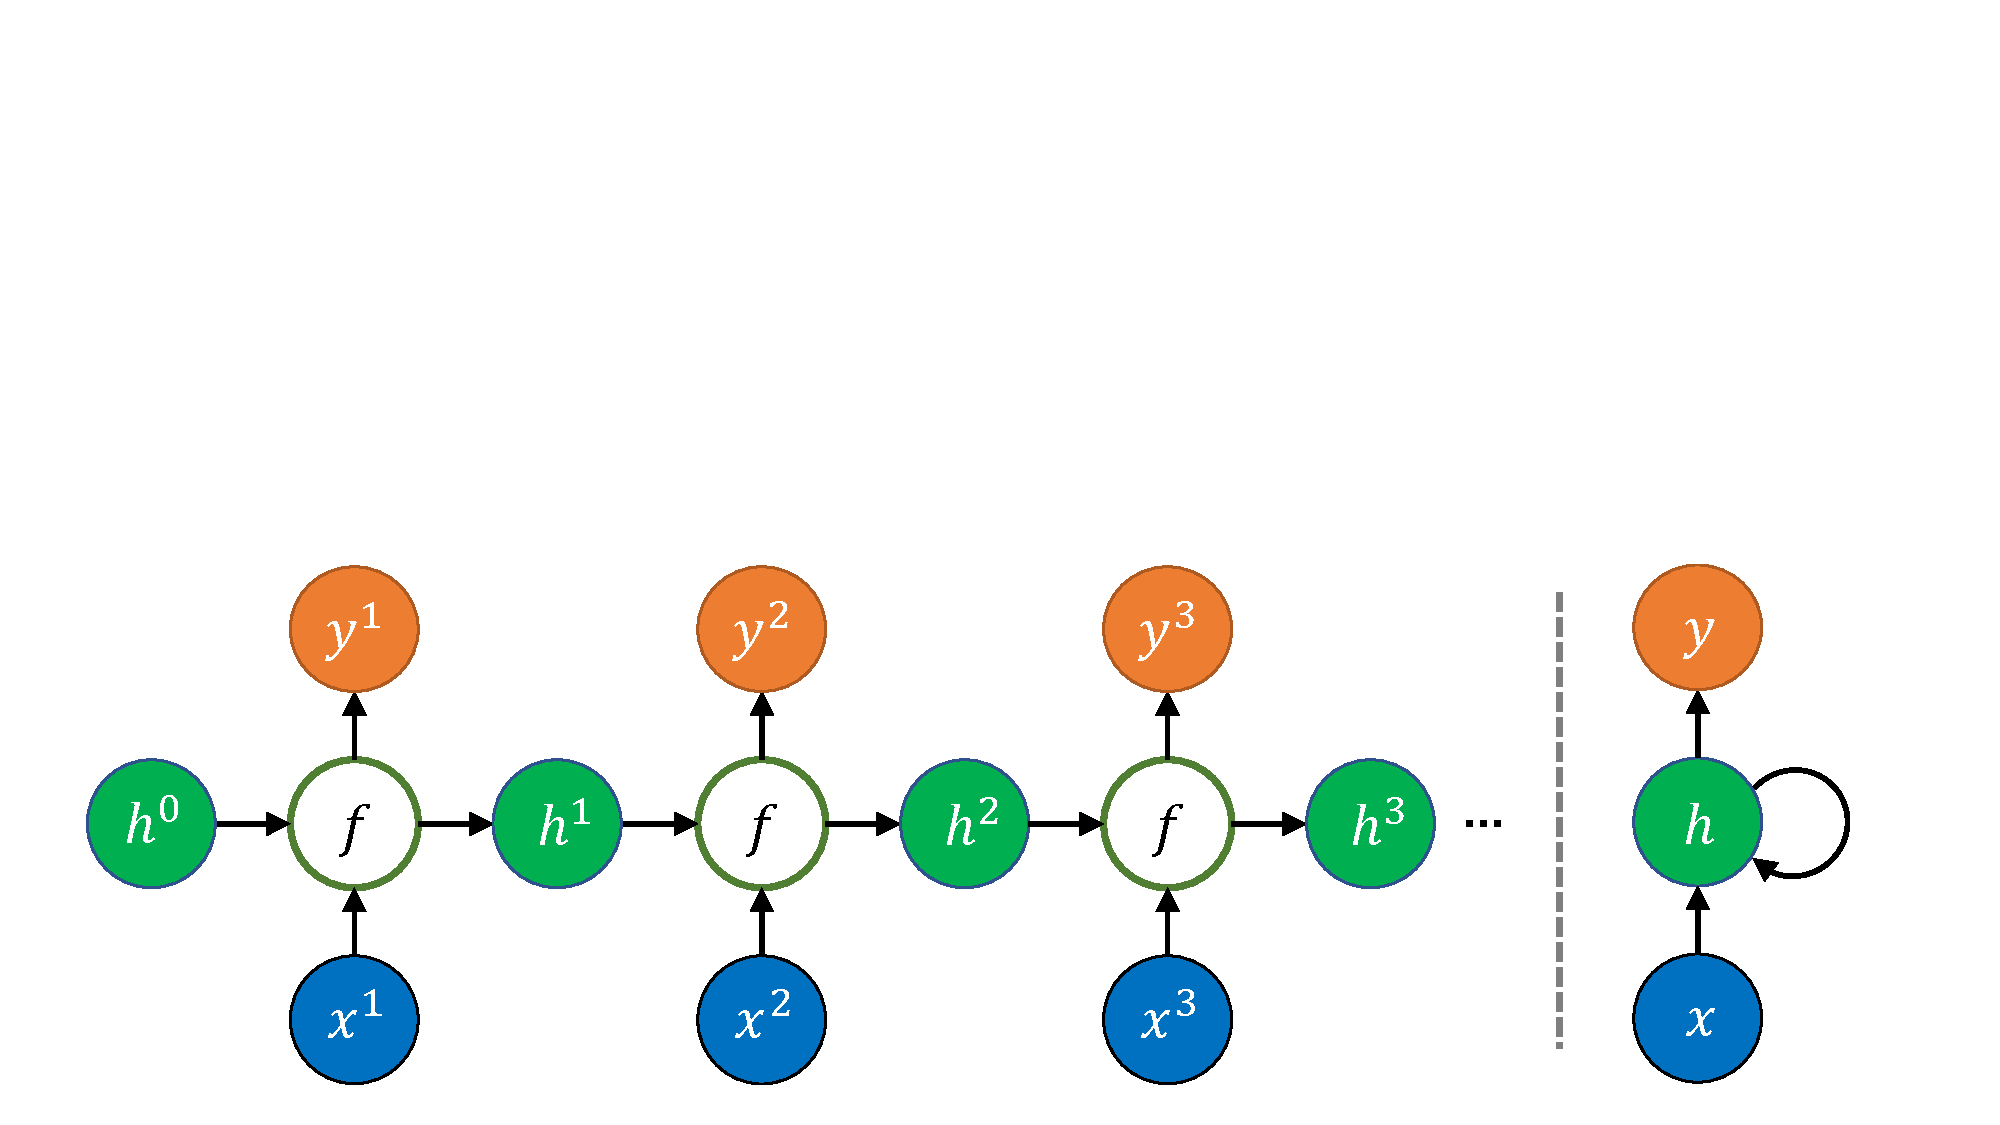
\includegraphics[width=\linewidth]{rnn2.pdf}
    \caption{循环神经网络}
    \label{rnn2}
\end{figure}


此外, 图\ref{rnn2}左为通用的RNN架构. 不同的应用场景下, 可以对其做各种灵活的调整. 
如, 对于文本分类的问题(如, 评论是否正面), 仅关心序列最后对应的节点输出即可. 如
图\ref{rnn3}所示. 此时输入-输出是{\bf 多对一}的关系. 对于输入为单个元素但输出为
序列的情况(即, 输入-输出是{\bf 一对多}, 如音乐生成), 则恰恰相反: 仅在一开始输入
单个元素, 对后续的多个循环节点提取输出即可. {\bf 多对多}分两种情形, 输入输出等长
时, 典型应用是命名实体识别(Name Entity Recognition);不等长时的常见应用则是机
器翻译. 特别地, 当输入、输出都不是序列时, RNN特化为一般的神经网络. 


\begin{figure}[!hbt]
    \center
    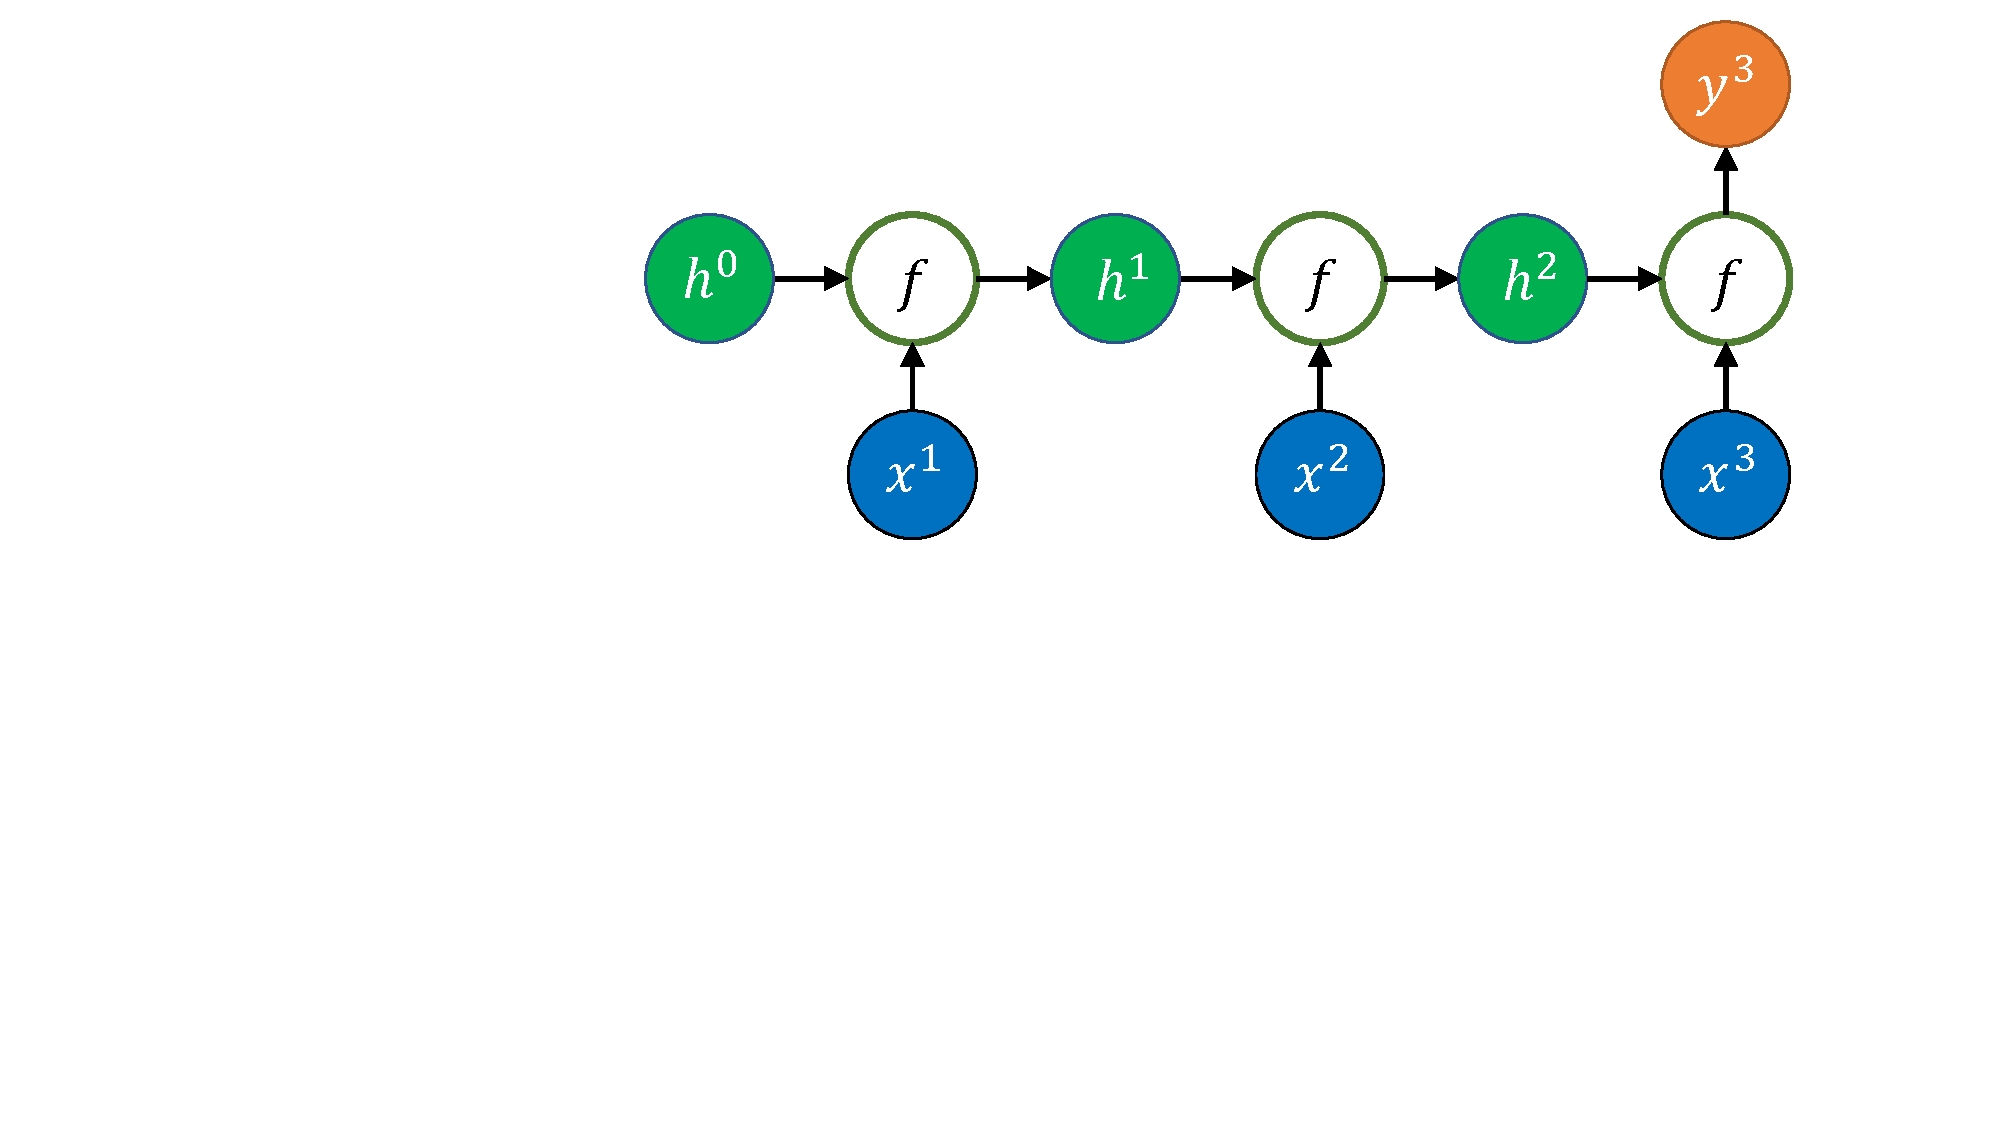
\includegraphics[width=.6\linewidth]{rnn3.pdf}
    \caption{序列到单输出的情形. $y=\sigma(W^3h^3 + b^3)$}
    \label{rnn3}
\end{figure}


Encoder-Decoder模型, 也称为Seq2Seq模型, 是RNN的一大变种, 如图\ref{rnn4}所示, 
它接受的输入和输出的序列不等长(如, 文本翻译). 它包含了两个RNN, 分别用于编码
和解码. 其中, $c$可以简单取编码器最后的隐状态$h^3$, 也可以取它的一种变换$q(h^3)$, 
还可以取所有隐状态的某种变换$q(h^1, h^2, h^3)$. $c$的维度大小代表了其能包含的信
息量. 



\begin{figure}[!hbt]
    \center
    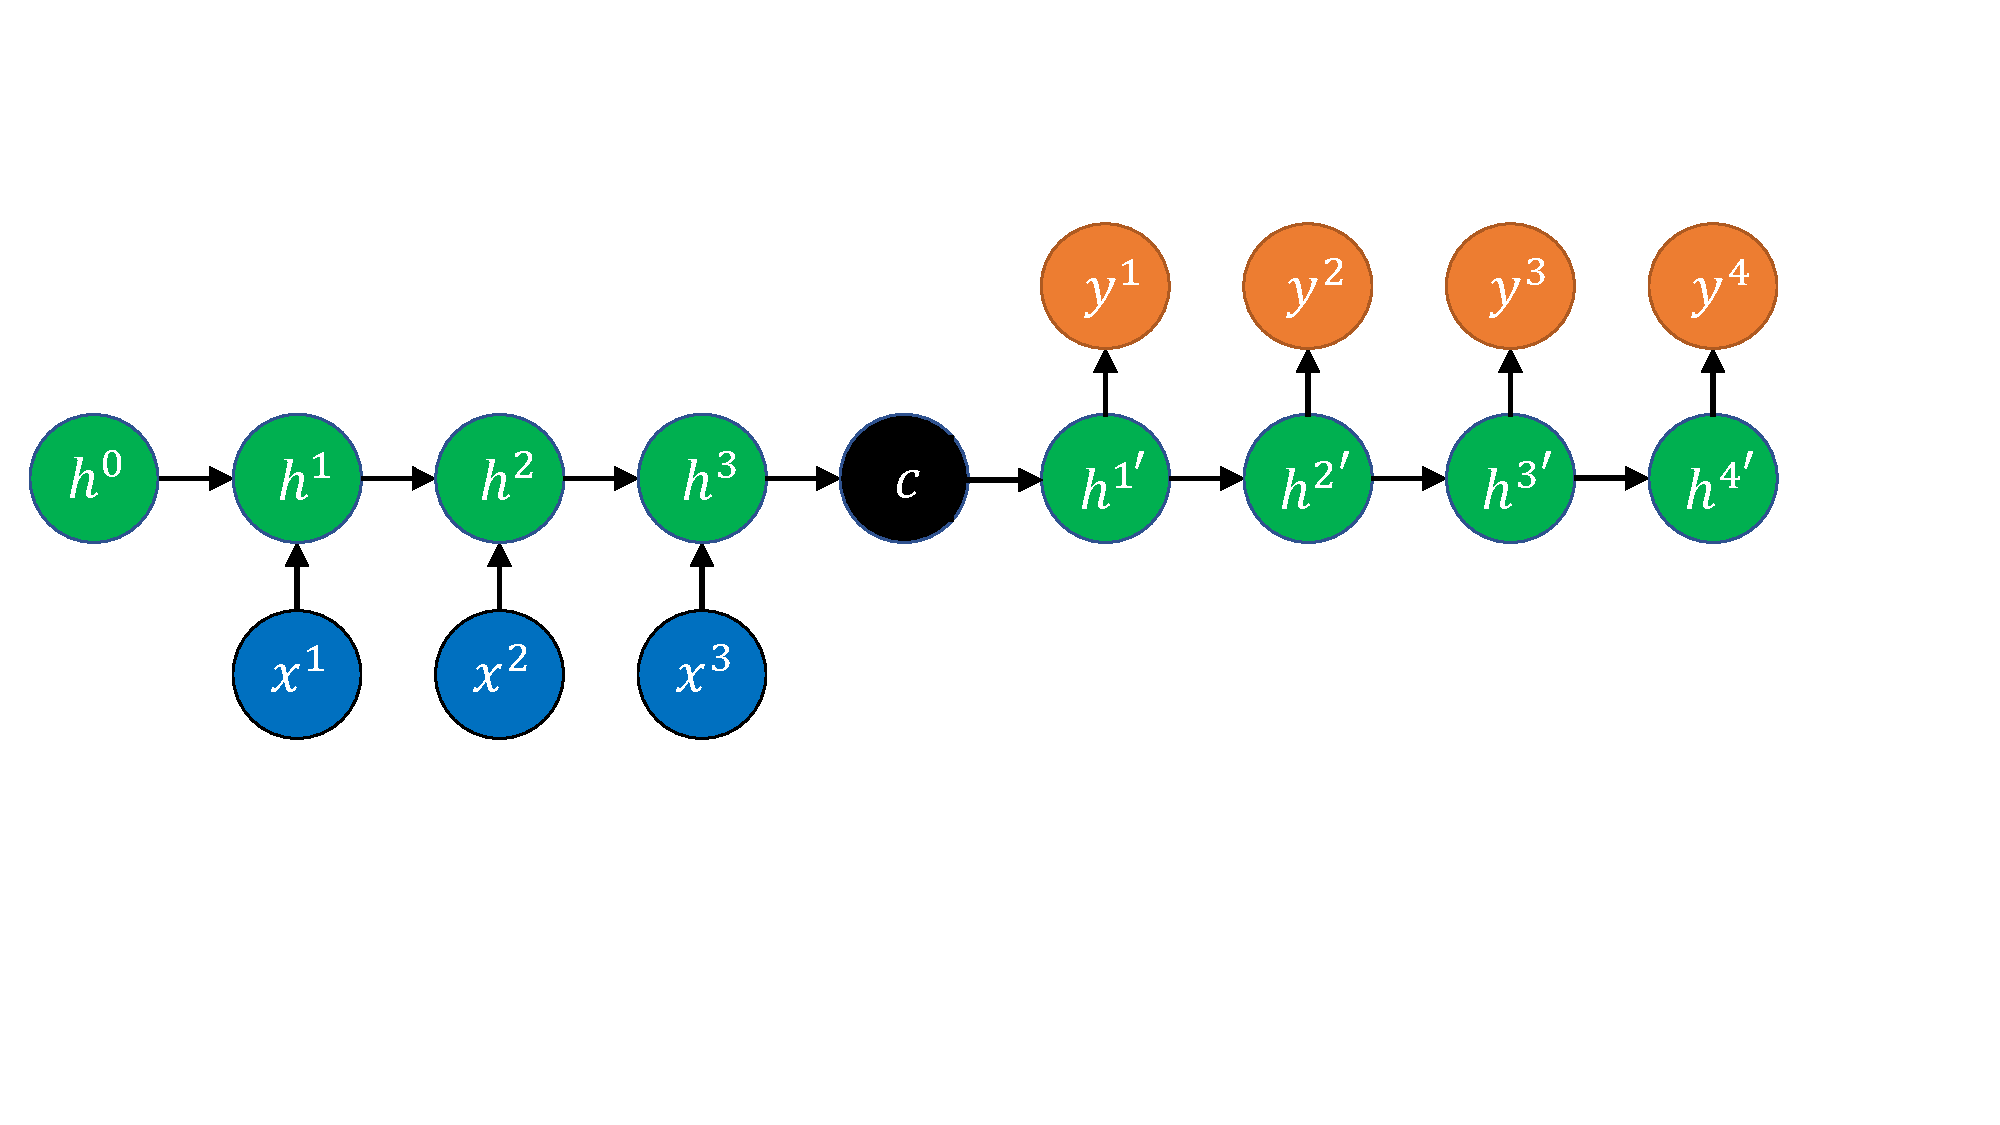
\includegraphics[width=.9\linewidth]{rnn4.pdf}
    \caption{Seq2Seq模型}
    \label{rnn4}
\end{figure}


\subsection{损失函数及训练}
RNN的损失函数是累加的, 它是各个时间节点的损失之和. 单个节点的损失后者可以是该点
输出序列与预测可以是该点输出序列与预测序列的距离, 如下式, 也可以是交叉熵. 


\begin{align}
\mathcal{L}(\widehat{y},y)\notag &= \sum_t \mathcal{L}(\widehat{y}^t, y^t)\\
                                  &= \sum_t c \Vert y^t - \widehat{y}^t \Vert^2
\end{align}


其中, $c=0.5$. 训练的目标是使$L$越小越好:

\begin{equation}
w^{new} = w - \gamma \frac{\partial L}{\partial w}
\end{equation}

其中, $\gamma$为学习率. $\frac{\partial L}{\partial w}$本质上是对$W^h$, $W^i$
以及$W^o$求偏导. 在不考虑激活函数的情形下, 一个具有三个隐含单元的RNN有:

\begin{align}
h^1 = W^h h^0 + W^i x^0\notag \\
h^2 = W^h h^1 + W^i x^1\notag \\
h^3 = W^h h^2 + W^i x^2
\end{align}


对最后一个隐含单元, 有$L^3 = 0.5 \Vert y^t - \widehat{y}^t \Vert^2$. 
计算其对各参数的偏导, 有:

\begin{equation}
\frac{\partial L^3}{\partial W^o} = \frac{\partial L^3}{\partial y^3}
\frac{\partial y^3}{\partial W^o}
\end{equation}

\begin{align}
\frac{\partial L^3}{\partial W^i} & = \frac{\partial L^3}{\partial y^3}
\frac{\partial y^3}{\partial h^3}\frac{\partial h^3}{\partial W^i}
\notag \\ & + \frac{\partial L^3}{\partial y^3}
\frac{\partial y^3}{\partial h^3}\frac{\partial h^3}{\partial h^2}
\frac{\partial h^2}{\partial W^i}
\notag \\ & + \frac{\partial L^3}{\partial y^3}
\frac{\partial y^3}{\partial h^3}\frac{\partial h^3}{\partial h^2}
\frac{\partial h^2}{\partial h^1}\frac{\partial h^1}{\partial W^i}
\end{align}

\begin{align}
\frac{\partial L^3}{\partial W^h} & = \frac{\partial L^3}{\partial y^3}
\frac{\partial y^3}{\partial h^3}\frac{\partial h^3}{\partial W^h}
\notag \\ & + \frac{\partial L^3}{\partial y^3}
\frac{\partial y^3}{\partial h^3}\frac{\partial h^3}{\partial h^2}
\frac{\partial h^2}{\partial W^h}
\notag \\ & + \frac{\partial L^3}{\partial y^3}
\frac{\partial y^3}{\partial h^3}\frac{\partial h^3}{\partial h^2}
\frac{\partial h^2}{\partial h^1}\frac{\partial h^1}{\partial W^h}
\end{align}


上述几个式子中, $\widehat{y}$为常数, 此外用到了求导的链式法则. 另外, $L^3$对
$W^s$的梯度为$L^3$对$W^s$在$t=1,2,3$的梯度之和, 这是因为$h^t$是随时间序列向前
传播的(后来者是前面取值的函数), 而$h^t$又是$W^h$和$W^i$的函数, 故此处求偏导
数需要追溯该时刻之前所有时刻的信息. 这种训练方法也称为BPTT
(back-propagation through time), 本质上就是一种BP梯度下降算法. 



这样, 在$t$时刻对$W^h$($W^i$同理)求偏导的公式即为\cite{3}

\begin{equation}
\frac{\partial L^t}{\partial W^h} = \sum_{k=1}^t 
\frac{\partial L^t}{\partial y^t}(\prod_{j=k+1}^{t} 
\frac{\partial h^{j}}{\partial h^{j-1}})\frac{\partial h^k}{\partial W^h}
\end{equation}

若激活函数为$tanh$时, 考虑到$h^t=tanh(W^i x^t + W^h h^{t-1})$, 则

\begin{equation}
\prod_{j=k+1}^{t} \frac{\partial h^{j}}{\partial h^{j-1}} =
\prod_{j=k+1}^{t} tanh^{\prime} W^h
\end{equation}

对于$tanh$, 恒有$tanh^{\prime} \leq 1$. 记$W$的最大特征值为$\lambda$, 则
$\lambda < 1$时, 会出现{\bf 梯度消失}的情况, 即, 较为久远的时间节点对后面输出
的影响(贡献)趋近于消失. 而当$\lambda$较大时, 多个大于1的项累乘会导致{\bf 梯度
爆炸}. 总而言之, 梯度消失/爆炸都是由于神经网络(时间上或空间上)的深度加深而
引起的\cite{4}. 



需要指出, 梯度消失或爆炸是不能从根本上解决的, 只能抑制. 使用$ReLU$作为激活函数
可以明显减缓这两种现象:该函数在负半轴导数为0, 正半轴则恒为1. 但$ReLU$也有可能
使得大量神经元无法激活, 需要合理设置偏置. 另一种解决梯度爆炸的思路是控制梯度在
某一门限内. 此外, 我们也可以理解: 深层神经网络中,有时候多加神经元的效果可能会
比多加深度好.



\subsection{其他注解}
RNN的优缺点如表\ref{trnn1}所示\cite{2}. 

\begin{table}
\caption{RNN的优缺点}
	\centering
	\small
	\begin{tabular}{ll}
	\toprule
    优势 & 缺陷\\
    \midrule
    \begin{minipage}[t]{.4\linewidth}
    \begin{itemize}[leftmargin=*]
        \item 处理任意长输入
        \item 模型不随输入增大
        \item 考虑历史信息
        \item 不同循环的时刻共享权重
    \end{itemize}
    \end{minipage} &
    \begin{minipage}[t]{.4\linewidth}
    \begin{itemize}[leftmargin=*]
        \item 难以并行, 计算较慢
        \item 久远的信息难以保留
        \item 对当前输入, 不考虑下文
    \end{itemize}
    \end{minipage} \\
    \bottomrule
	\end{tabular}
	\label{trnn1}
\end{table}



\section{LSTM}
长短期记忆(Long Short-Term Memory, LSTM)是一种特殊的RNN, 针对长序列训练过程中
的梯度消失和梯度爆炸问题而提出. LSTM结构和普通RNN的主要区别如图\ref{lstm1}所示. 

\begin{figure}[!hbt]
    \center
    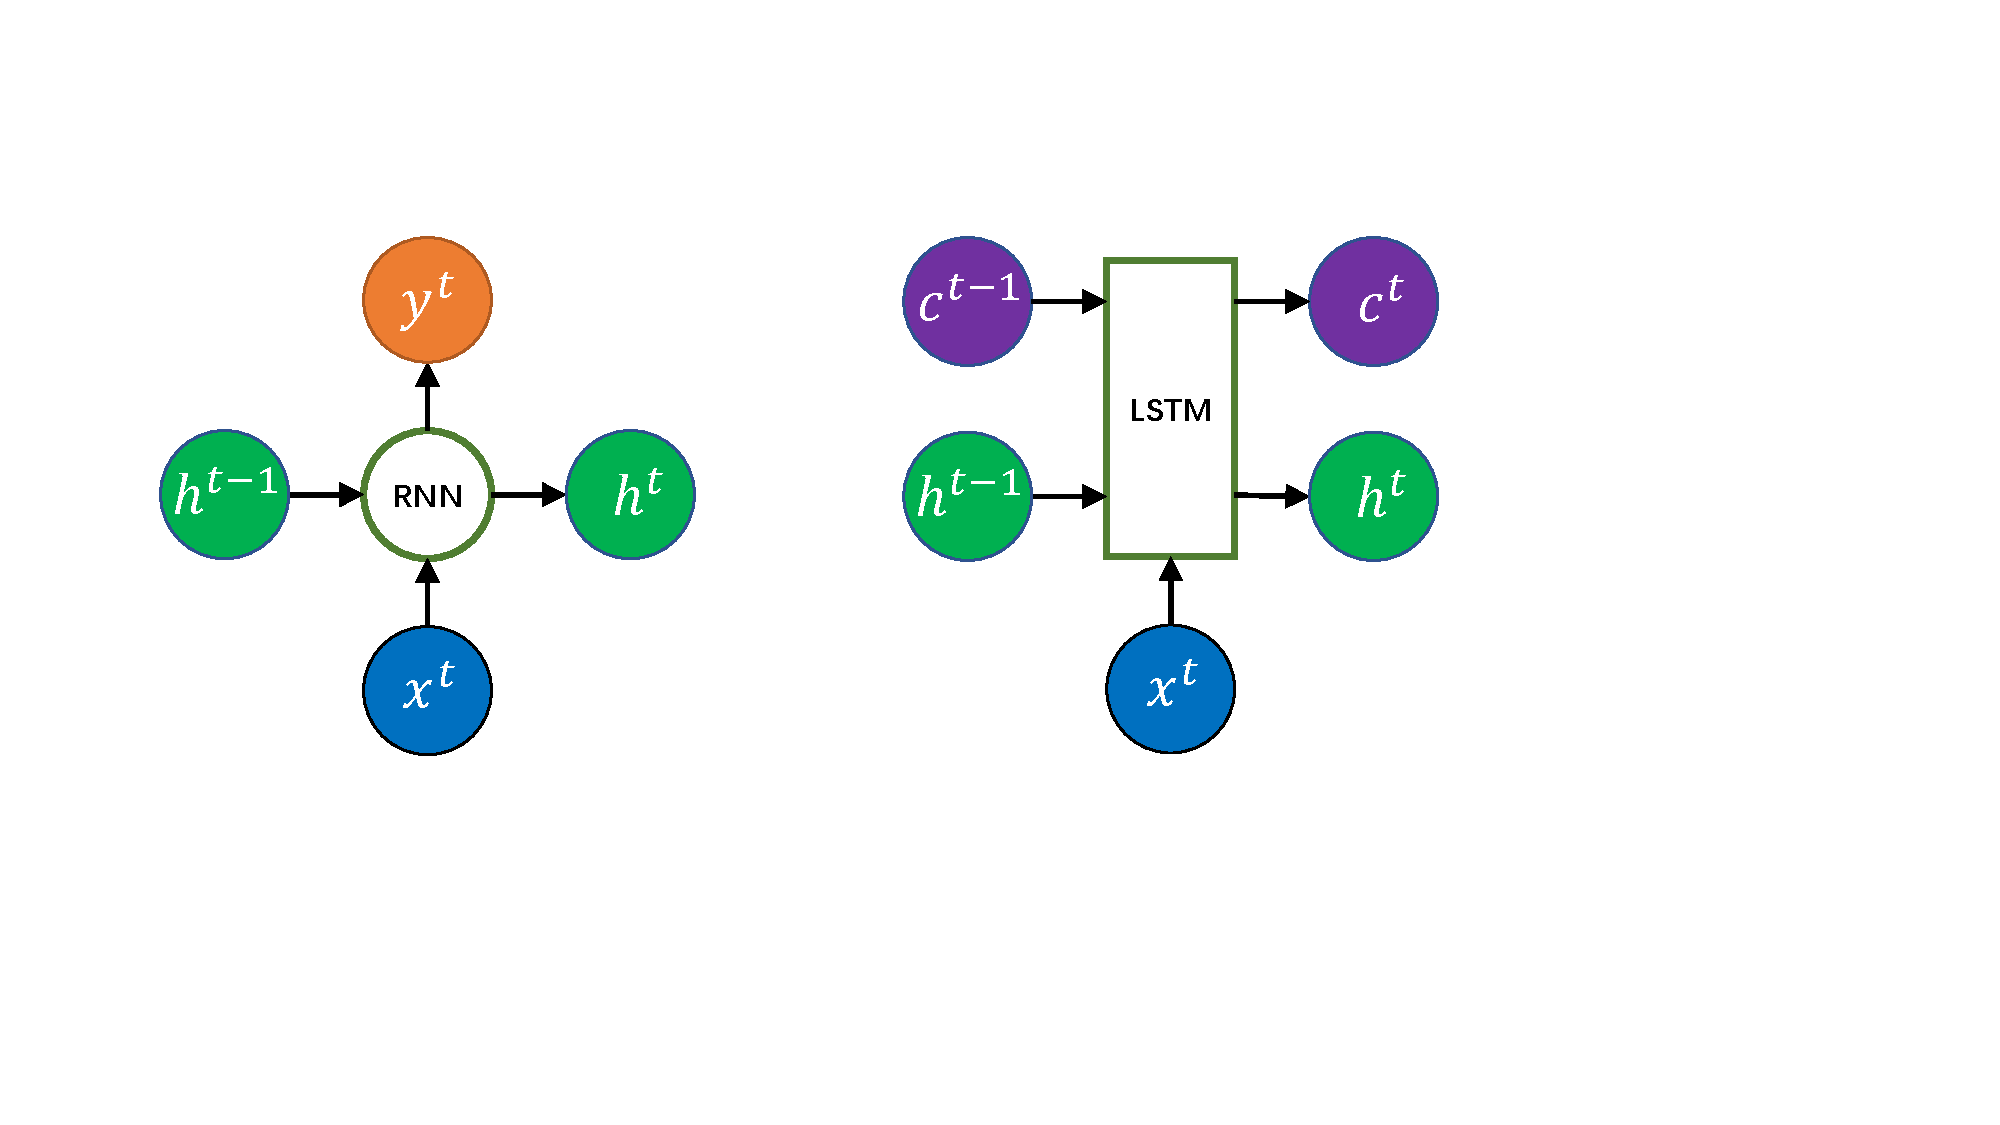
\includegraphics[width=0.8\linewidth]{lstm1.pdf}
    \caption{LSTM基本单元}
    \label{lstm1}
\end{figure}

相比RNN只有一个传递状态$h^t$(hidden state), LSTM额外添加了一个$c^t$(cell 
state, 单元状态). LSTM中, 信息在单元间顺序传递, $c^t$的作用相当于RNN中的$h^t$. 
LSTM通过门(gate)来控制丢弃或者增加信息, 从而实现遗忘或记忆的功能. ``门''是一种使
信息选择性通过的结构, 由一个$sigmoid$函数和一个点乘操作组成: 故输出值在$[0,1]$
区间(0代表完全丢弃, 1代表完全通过). 一个LSTM单元有三个这样的门, 分别是遗忘门
(forget gate), 输入门(input gate)和输出门(output gate)\cite{1}.



\subsection{LSTM的三个门}
{\bf 遗忘门}. 遗忘门拼接上一个单元的输出和本单元的输入作为输入, 其输出$z^f$
表征(控制)上一个单元状态$c^{t-1}$被遗忘的程度.

\begin{equation}
z^f=\sigma(W^f[h^{t-1},x^t])
\end{equation}

{\bf 输入门}. 这个阶段对输入有选择性地进行记忆, 与一个$tanh$函数配合, 控制
有哪些新信息被加入. 当前的输入内容表征为

\begin{equation}
\widetilde{c}^t=tanh(W^c[h^{t-1},x^t])
\end{equation}

而选择的门控信号则是由$z^i$来进行控制:

\begin{equation}
z^i=\sigma(W^i[h^{t-1},x^t])
\end{equation}

则输入门总的输出, 即当前时间输入的新信息, 为$z^i \odot \widetilde{c}^t$. 其中, 
$\odot$表示矩阵元素间的乘法. 现在, 综合遗忘门的输出(上一单元被遗忘的程度)和
输入门的输出(本单元新信息加入的程度), 即可得到传输给下一个时间节点的新单元状态
$c^{t+1}$.

\begin{equation}
c^{t+1}=z^f \odot c^t + z^i \odot \widehat{x}^t
\end{equation}


{\bf 输出门}. 输出门控制当前的单元状态有多少被过滤掉. 

\begin{align}
h^t &= z^o \cdot tanh(c^t) \\
\text{where} \quad z^o &= \sigma(W^o[h^{t-1},x^t])
\end{align}

与普通RNN类似, 输出$y^t$直接取$h^t$或它的某种变换\footnote{一种做法是, 
$y^t=\sigma(W^{\prime}h^t)$, 但这又增加了参数量. 简单起见, 本文中相关的示意图
中, 视$y^t$与$h^t$等价}. 相比RNN, LSTM更擅长处理长序列任务, 但代价是参数变多, 
训练难度加大. 



综上, LSTM中一个基本单元的内部结构如图\ref{lstm2}所示. 其中, $\Gamma^f$, 
$\Gamma^i$和$\Gamma^o$分别代表遗忘门, 输入门和输出门.


\begin{figure*}[!hbt]
    \center
    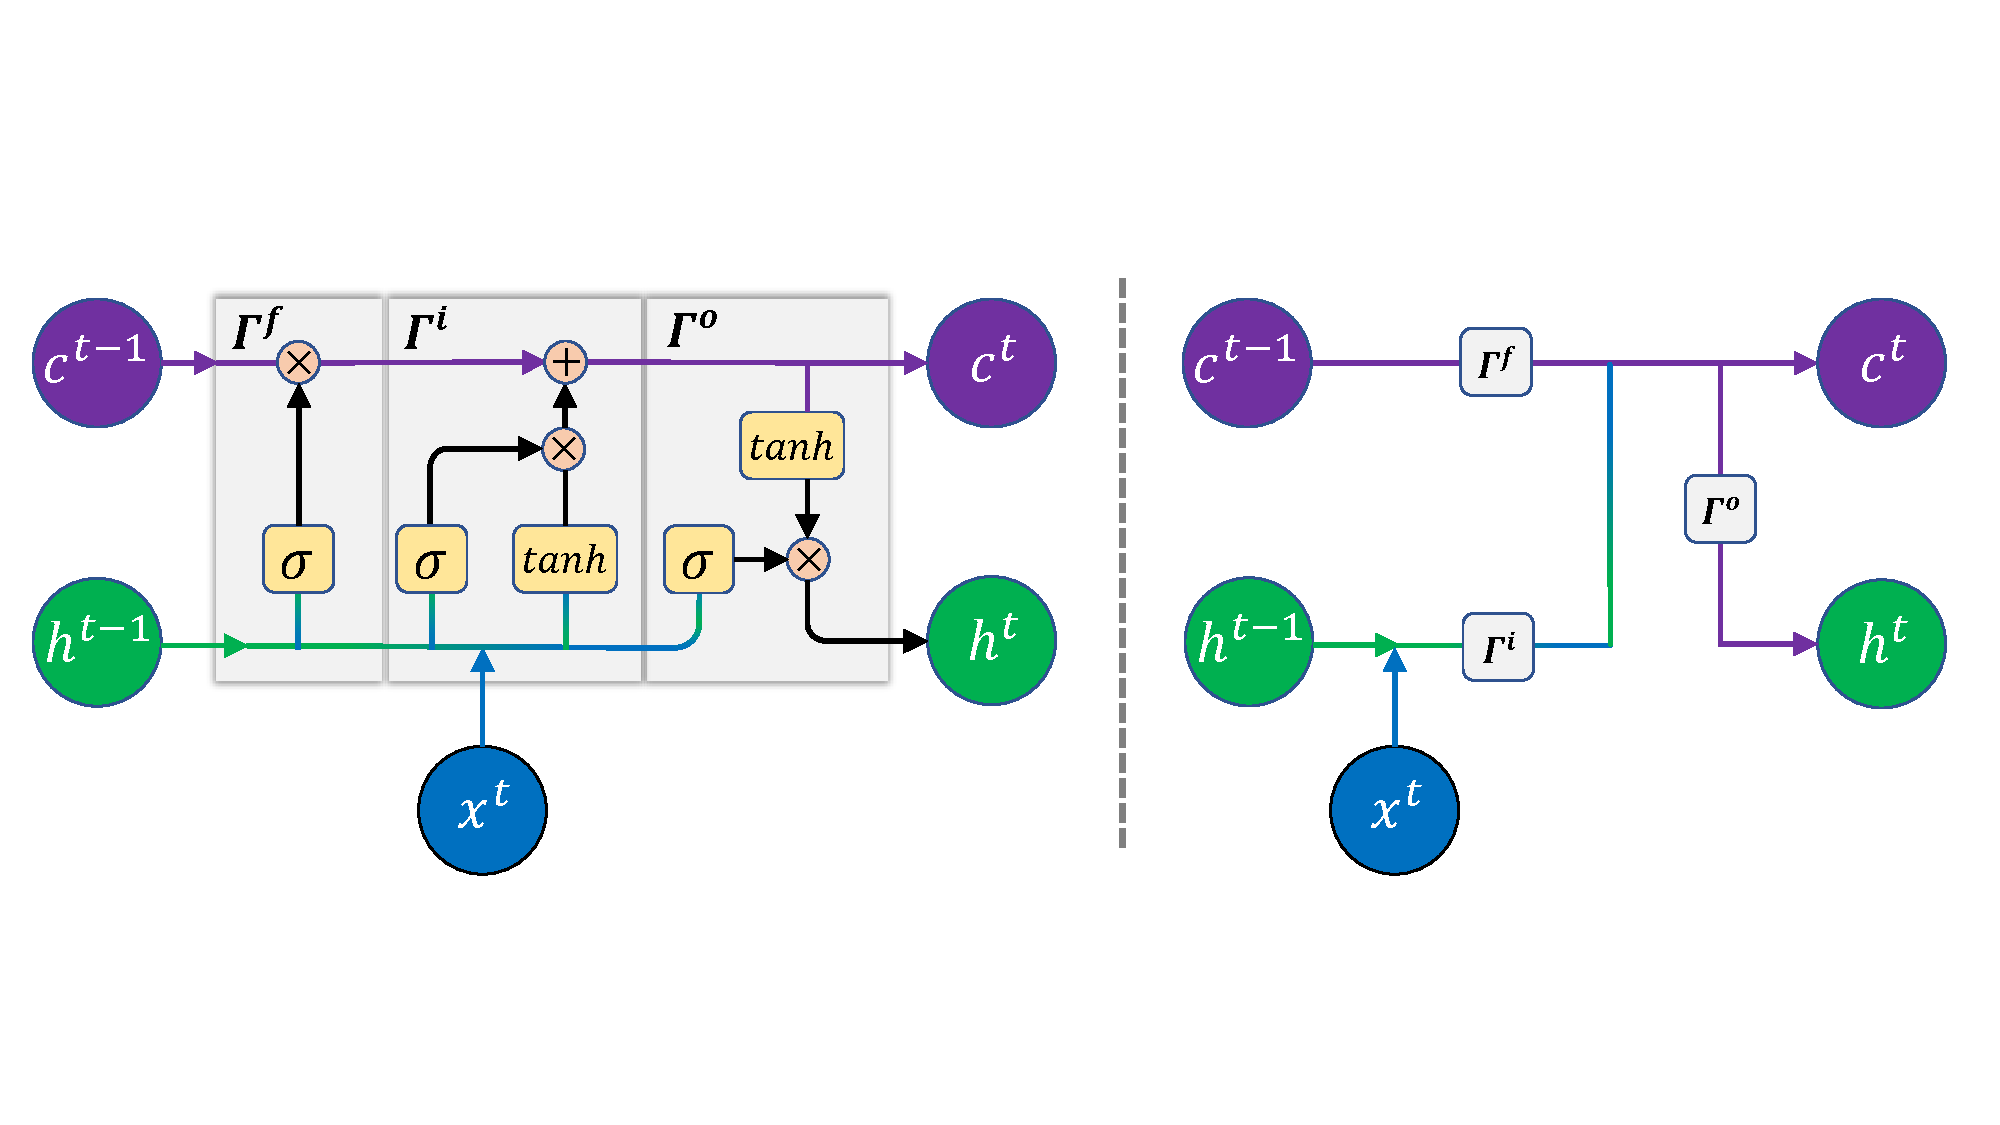
\includegraphics[width=.8\linewidth]{lstm2.pdf}
    \caption{LSTM基本单元内部结构}
    \label{lstm2}
\end{figure*}

\subsection{其他注解}
$c^t$是对前期记忆和当前输入的线性变换($c=ax+by$), 而$h^t$则是$c^t$经过门控
选择的信息. $sigmoid$的选取遵循了很简单的原则: 令输出值落在$[0,1]$区间内.
但是, 它不适合直接用作对数据的处理. 一个问题是, 它的输出不是以0为中心的. 相对
来说, 我们更希望当函数的输入是0时, 输出也为0(这对加快收敛有利). 故可以选取$tanh$
提供对数据的非线性处理. 此外, $tanh$的导数范围比$sigmoid$更大(最小值都为0, 但后
者的梯度上限是0.25, 而前者为1), 一般来说收敛会更快, 梯度消失也更慢. 当然, 为了
进一步克服梯度消失, 改善收敛速度, 也可以考虑将其更换为$ReLU$等激活函数.


\section{GRU}
LSTM参数量较大, 故在实际应用中门控循环单元GRU(Gated Recurrent Unit)\cite{5}得到
了人们的青睐. GRU是LSTM的一种特例, 参数量更小, 但效果接近. GRU只有两个门: 重置门
(reset gate)与更新门(update gate). 重置门控制输入与前面的记忆相结合的程度, 类比
于LSTM的选择记忆(输入门); 更新门则类比于LSTM的遗忘门与输出门, 控制保留前面记忆的
程度\footnote{特别地, 当重置门为1, 更新门为0时, 得到的即是标准的RNN模型\cite{6}}.



{\bf 重置门}. 首先, 重置门对传入的前一个隐含状态$h^{t-1}$进行``重置''得到
$\widetilde{h}^{t-1}$, 再将其与输入$x^t$拼接, 并使用$tanh$放缩至$[-1,1]$:

\begin{align}
r^t &=\sigma(W^r[h^{t-1},x^t]) \label{eq} \\
\widetilde{h}^{t-1} &= r^t \odot h^{t-1} \\
h^{t\prime} &= tanh(W \widetilde{h}^{t-1}, x)
\end{align}



得到的$h^{t\prime}$相当于LSTM选择记忆(输入门)的输出\footnote{对形如\ref{eq}的
式子, 很多资料中也将它们展开为形如$r^t=\sigma(W^r x^t+U^r h^{t-1})$的形式. 
本质上,两个变量的线性组合可以表示为它们的拼接再element-wise与一个矩阵相乘(分块
矩阵). 故为了简化表达, 全文中均取这种简化形式(前面的LSTM亦如此)}.


{\bf 更新门}. 更新门控的值由下式给出, 与前面的各个门控值的计算方式完全相同:

\begin{equation}
z^t =\sigma(W^z[h^{t-1},x^t])
\end{equation}

GRU的简练之处就在于, 这一门控可以同时代表记忆与遗忘. 当前时间节点隐含层的输出
记为:

\begin{equation}
h^t = (1-z^t) \odot h^{t-1} + z^t \odot h^{t\prime}
\end{equation}

式中, 相加的前后两项分别表示对原隐藏状态的选择性遗忘以及对当前节点信息的选择性
记忆.

\section{注意力模型}
对于前述的Encoder-Decoder模型,存在的一个问题是: 对于一个特定任务, 输入给Decoder
的编码$C$是固定的, 故对于输出的不同元素($y^1=f(C), y^2=f(C, y^1), y^3=f(C, y^1, 
y^2), ...$), 同一个输入元素对它们的影响并没有特别的差异. 也就是说, 模型只是泛泛
地接受输入, 但不会像人一样会特别关注某些更为重要的部分.



为了让模型能够对输入的特定部分付出额外的注意力以提升表现, 人们提出的注意力模型
(Attention Model, AM)为每个输出单独计算各个输入元素对其影响的权重. 此时, 
$y^1=f(c^1), y^2=f(c^2, y^1), y^3=f(c^3, y^1, y^2), ...$, 其中$c_i$体现了输入的
不同元素对当前输出影响力的概率分布, 是输入各元素对应RNN状态的加权求和. 实践证
明, 注意力模型既能克服RNN输入长度增加带来的性能下降问题, 也能用于提高神经网络的
可解释性\cite{8}. $c^t$由下式给出

\begin{equation}
c^t = \sum_{k=1}^{L_x}\alpha^{tk}h^k, \text{where} \sum_k \alpha^{tk} = 1
\end{equation}

其中, $L_x$是输入序列的长度. 模型输出$y^t$时应对输入$h^k$付出的注意力
$\alpha^{tk}$由下式(类似$softmax$)进行归一化, 使得$\sum_k \alpha^{tk} = 1$, 同时
$exp$使得重要的项更加凸显

\begin{equation}
\alpha^{tk} = \frac{exp(e^{tk})}{\sum_{n=1}^{L_x} exp(e^{tn})}
\end{equation}

式中, $e^{tk}$是模型输出$y^t$与对输入$h^k$的``相似度'', 可以根据多种方式计算得
到, 常见的算法有向量点积, 余弦相似度等, 也可以通过多层感知机等学习算法
求得\cite{9}.

\begin{thebibliography}{99}
\bibitem{1}
Understanding LSTM Networks. \url{http://colah.github.io/posts/2015-08-Understanding-LSTMs/}
\bibitem{2}
cs-230: cheatsheet-recurrent-neural-networks. \url{https://stanford.edu/~shervine/teaching/cs-230/cheatsheet-recurrent-neural-networks}
\bibitem{3}
RNN梯度消失和爆炸的原因. \url{https://zhuanlan.zhihu.com/p/28687529}
\bibitem{4}
漫谈RNN之梯度消失及梯度爆炸. \url{http://bbs.imefuture.com/article/4405}
\bibitem{5}
Chung J, Gulcehre C, Cho K H, et al. Empirical evaluation of gated recurrent neural networks on sequence modeling[J]. arXiv preprint arXiv:1412.3555, 2014.
\bibitem{6}
经典必读:门控循环单元(GRU)的基本概念与原理. \url{https://www.jiqizhixin.com/articles/2017-12-24}
\bibitem{7}
RNN. \url{https://blog.csdn.net/zhaojc1995/article/details/80572098}
\bibitem{8}
An Attentive Survey of Attention Models. \url{https://arxiv.org/abs/1904.02874}
\bibitem{9}
深度学习中的注意力模型. \url{https://zhuanlan.zhihu.com/p/37601161}
\end{thebibliography}

\end{document}


